\documentclass[a4paper,12pt]{article}
\usepackage[a4paper, margin=2.5cm]{geometry}
\usepackage[pdftex]{graphicx}
\usepackage{tikz}
\usepackage{pgfplots}
\usepackage{enumitem}
\usepackage{float}
\usepackage[document]{ragged2e}
\usepackage[utf8]{inputenc}
\usepackage[T1]{fontenc}
\usepackage[spanish,es-tabla]{babel}
\renewcommand{\shorthandsspanish}{}
\usepackage{xurl}
\usepackage{lipsum}
\usepackage{mwe}
\usepackage{multirow}
\usepackage{multicol}
\usepackage{siunitx}
\usepackage{listings}
\usepackage{circuitikz}
\usepackage{tabularray}
\usepackage{amsmath}
\usepackage{gensymb}


\usetikzlibrary{arrows.meta,bending}
\graphicspath{ {/home/saikkopat/Documents/ESCOM/FDD/P03/IMG/} }

\usepackage[none]{hyphenat}

\begin{document}

\begin{titlepage}
	\begin{tikzpicture}[overlay, remember picture]
		\path (current page.north east) ++(-0.3,-1.8) node[below left] {
\includegraphics[width=0.35\textwidth]{/home/saikkopat/Documents/LOGOS IPN/EscudoESCOM}};
	\end{tikzpicture}
	\begin{tikzpicture}[overlay, remember picture]
		\path (current page.north west) ++(1.5,-1) node[below right] {
\includegraphics[width=0.2\textwidth]{/home/saikkopat/Documents/LOGOS IPN/logo}};
	\end{tikzpicture}
	\begin{center}
		\vspace{-1.5cm}
		{\LARGE Instituto Politécnico Nacional\par}
		\vspace{.5cm}
		{\LARGE Escuela Superior de Cómputo\par}
		\vspace{.5cm}
		{\Large Departamento de\\Ingeniería en Sistemas Computacionales\par}
		\vspace{2cm}
		{\large Unidad de aprendizaje:}\\{\Large Fundamentos de diseño digital\par}
		\vspace{2cm}
		{\scshape\Huge Práctica 3\par}
		{\itshape\Large Minimización usando mapas de Karnaugh\par}
		\vfill
		\vspace{.7cm}
		{\Large Equipo 2\par}
		\vspace{.7cm}
		{\Large Grupo: 3CV2\par}
		\vspace{.7cm}
		{\Large Integrantes:\\González Cárdenas Ángel Aquilez\\Hernández Reyes Diego Alberto\par}
		\vspace{1cm}
		{\Large Profesor: Barrón Vera Josué Emanuel\par}
		\vspace{1cm}
		{\large Fecha de realización: 25 de septiembre de 2023\par}
		{\large Fecha de entrega: 2 de octubre de 2023\par}
		\vfill
	\end{center}
\end{titlepage} 

\newpage

\tableofcontents

\newpage

\usepgfplotslibrary{units}

El alumno será capaz de diseñar un circuito lógico óptimo a partir del planteamiento de un problema,
utilizando el método de simplificación conocido para obtener la expresión lógica que determina al
circuito más simple. Comprobará también la efectividad de esos métodos al armar el circuito original y
el circuito simplificado.\par

\section*{Objetivo}

\textbf{Objetivos particulares}: \\Determinar la tabla de verdad representativa de un circuito lógico a partir del planteamiento de un problema.\\
Obtener, a partir de la tabla de verdad, la expresión lógica que describe el circuito y armarlo. \\
Obtener la forma simplificada de la expresión lógica y armar el circuito correspondiente, con la finalidad
de comprobar la equivalencia funcional de ambos circuitos.\par

\vspace{.5cm}

Los alumnos utilizarán los siguientes materiales y equipo:

\begin{multicols}{2}
\textbf{Equipo}\\
\begin{itemize}[nosep]
		\item \texttt{1 Dip switch de ocho interruptores}
\end{itemize}

\columnbreak

\textbf{Material}\\
\begin{itemize}[nosep]
		\item \textit{Protoboard}
		\item Software de simulacion
	
\end{itemize}

\end{multicols}


%
%
%		DESAROLLO
%
%


\section{Desarrollo}

\subsection{Planteamiento de la problematica}

A partir del planteamiento del siguiente enunciado, se determinó la tabla de verdad y el
circuito lógico que satisface la necesidad que se plantea:\par

\begin{quotation}
	En un laboratorio químico se elaboran 2 distintas soluciones a partir de las sustancias $A, B, C, D$ y $E$.\\
Estas sustancias pesan respectivamente: $160, 80, 40, 20$ y $10$ mg. Las soluciones son depositadas en
frascos que se transportan por medio de una banda hasta una báscula. Si el peso indicado en la báscula es
uno de los siguientes: $10, 20, 40, 60, 70, 90, 130. 150 160, 170, 220, 230, 240, 250, 260$ y $310$ mg,
entonces el dispositivo $F$, sellará el frasco y lo apartará de la banda; de otro modo, el frasco permanece
abierto y la banda lo transporta hacia otra etapa del proceso. Por las condiciones previas del proceso, no
es posible que lleguen a la báscula ni frascos vacíos ni frascos que contengan las siguientes soluciones $B,
BD, AD, ADE, AC$ y $ABCE$; todas las demás soluciones si pueden llegar hasta la báscula.\\
Se diseñará un circuito lógico que tenga como entradas las variables $A, B, C, D$ y $E$, tomando el valor de
1 lógico cuando la sustancia esté presente en la solución del frasco y 0 lógicos cuando no esté en la
solución. La salida será $F$, siendo 1 cuando la solución tenga uno de los pesos especificados y 0 cuando
tenga un peso diferente. Se deben considerar las condiciones irrelevantes del proceso.\par
\end{quotation}

\subsection{Tabla de verdad}

A partir de la problematica planteada en la seccion anterior, se determinó la tabla de verdad equivalente para los casos particulares, así como aquellos cuya salida no es relevante para el circuito.\\

\vspace{1cm}

\begin{figure}[ht!]
	\centering

	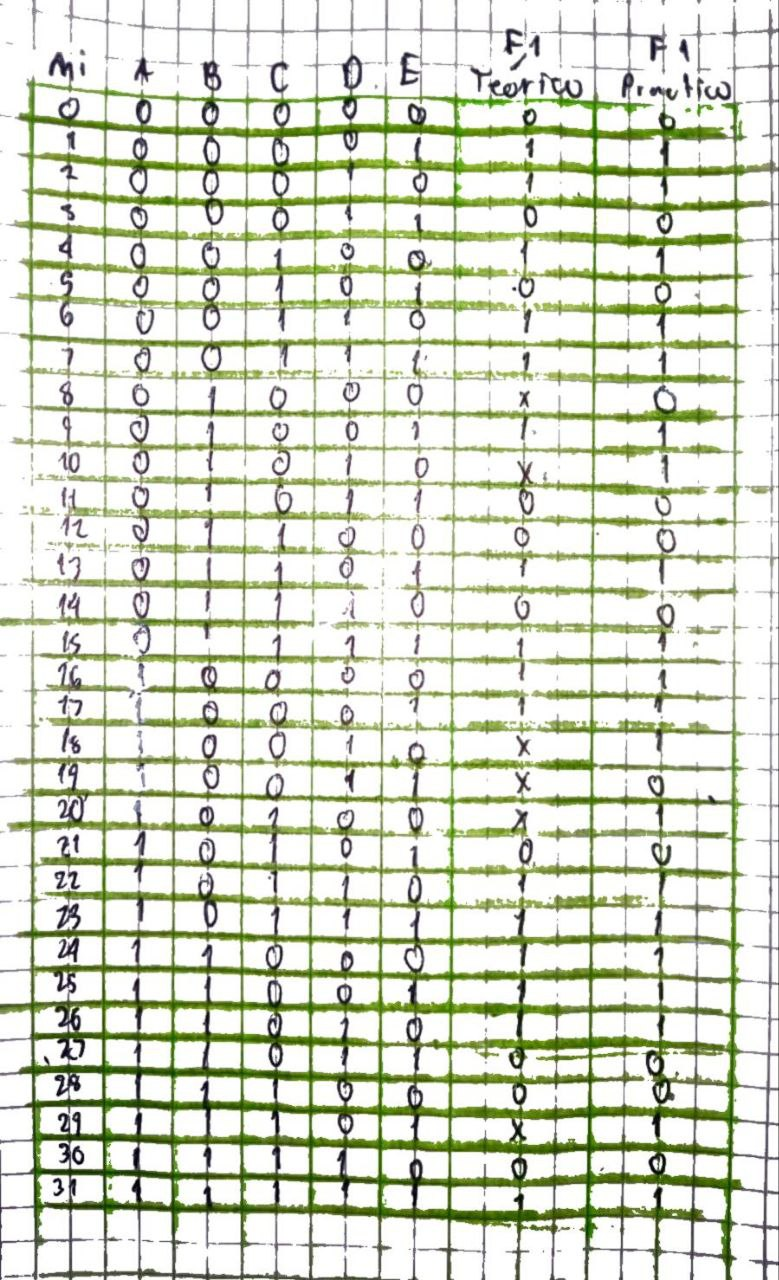
\includegraphics[width=.65\textwidth]{TAB01}

	\caption{Tabla de verdad para el circuito resultante}
\end{figure}

De modo que la funcion para cuyos valores es positivo el resultado queda compuesto por 16 resultados positivos y 6 terminos no relevantes, la simplificación mediante la suma de miniterminos correspondiente se vuelve una tarea tediosa y propensa a errores.\par

\newpage

\section{Simplificación mediante mapas de Karnaugh}

Para determinar una expresion equivalente con la menor cantidad de terminos posibles, se utilizó el siguiente mapa de Karnaugh, y al combinar los términos que no mantienen sus valores contantes se llegó a lo siguiente:\\

\begin{figure}[ht!]
	\centering

	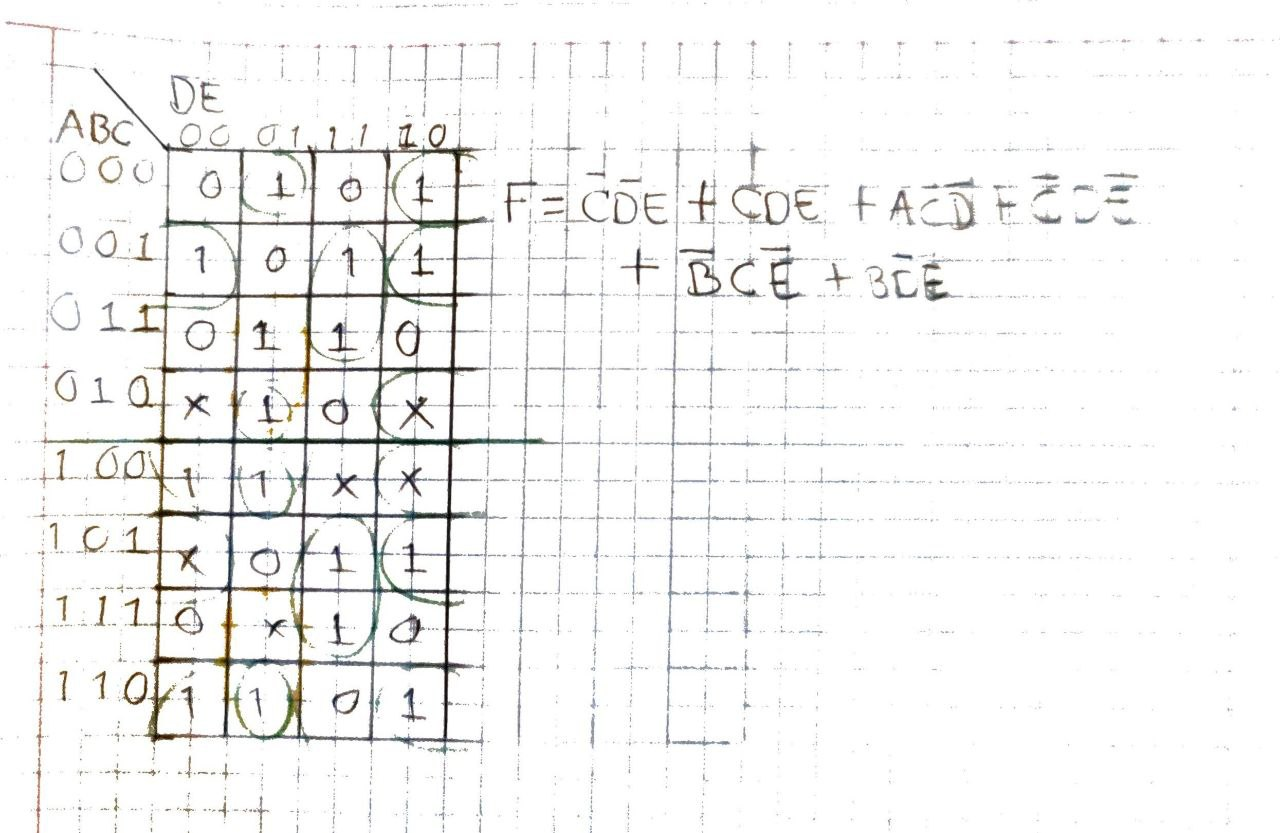
\includegraphics[width=.7\textwidth]{KNG}

	\caption{Mapa de Karnaugh utilizado}
\end{figure}

De modo que al dibujar el circuito con compuertas lógicas tenemos el siguiente circuito:

\begin{figure}[ht!]
	\centering

	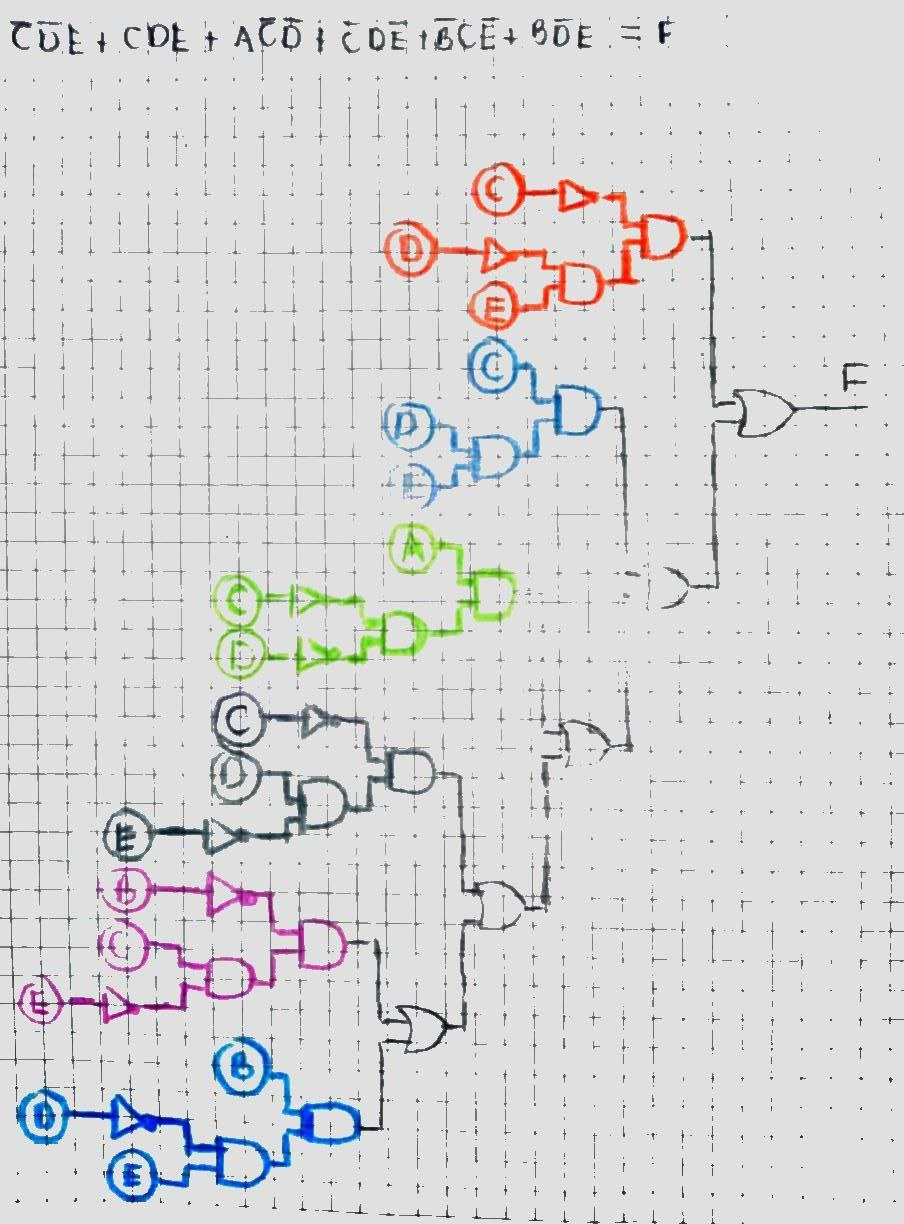
\includegraphics[width=.5\textwidth]{CIC}

	\caption{Circuito obtenido a partir de la simplificación}
\end{figure}


\subsection{Simulación del circuito}

Los resultados teoricos se comprobaron mediante la simulacion del circuito y quedaron registrados en el apartado de resultados teoricos de la tabla de verdad.\\


\begin{figure}[ht!]
	\centering

	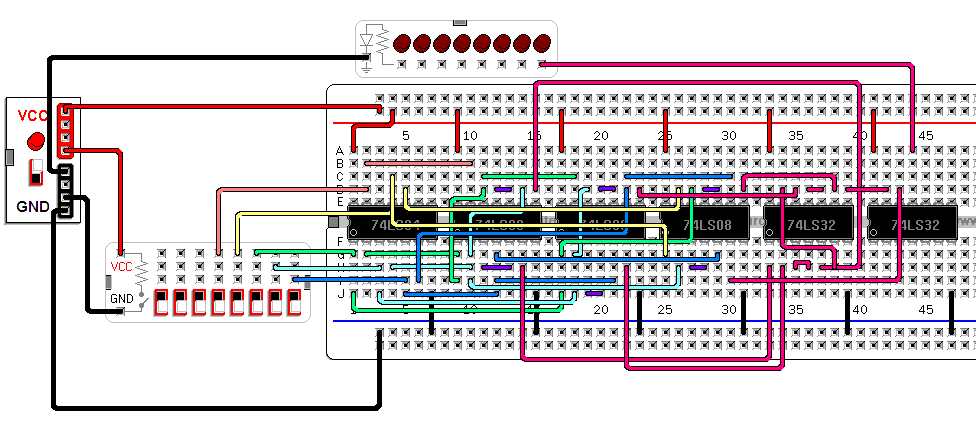
\includegraphics[width=.65\textwidth]{S0}

	\caption{\# 0 Entradas: 0,0,0,0,0 Salida: 0}
\end{figure}

\vspace{.5cm}

\begin{figure}[ht!]
	\centering

	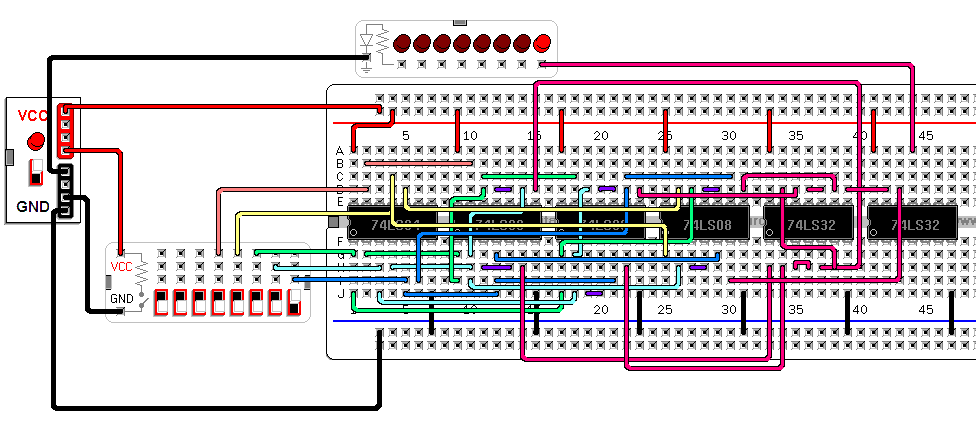
\includegraphics[width=.65\textwidth]{S1}

	\caption{\# 1 Entradas: 0,0,0,0,1 Salida: 1}
\end{figure}

\vspace{.5cm}

\begin{figure}[ht!]
	\centering

	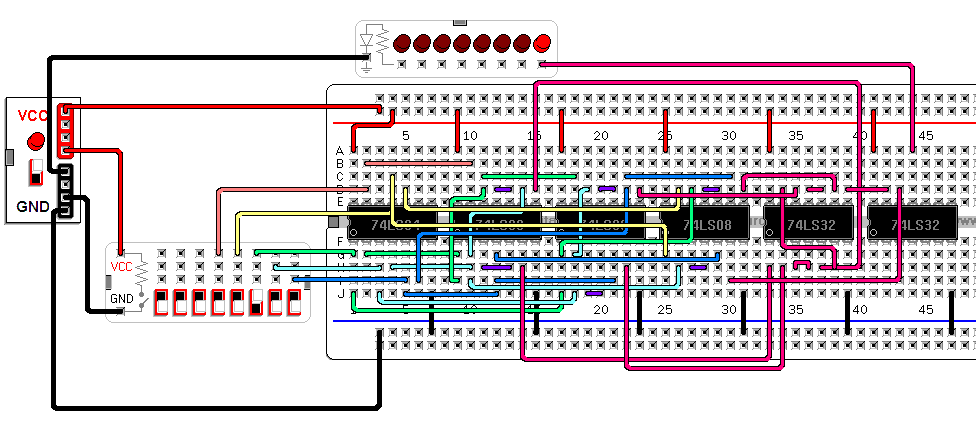
\includegraphics[width=.65\textwidth]{S4}

	\caption{\#4 Entradas: 0,0,1,0,0 Salida: 1}
\end{figure}

\vspace{.5cm}

\begin{figure}[ht!]
	\centering

	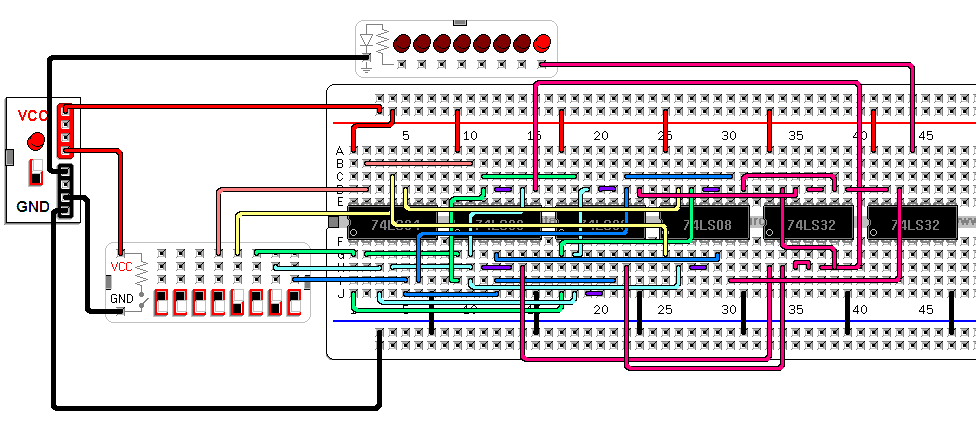
\includegraphics[width=.65\textwidth]{S10}

	\caption{\#10 Entradas: 0,1,0,1,0 Salida: 1}
\end{figure}

\vspace{.5cm}

\begin{figure}[ht!]
	\centering

	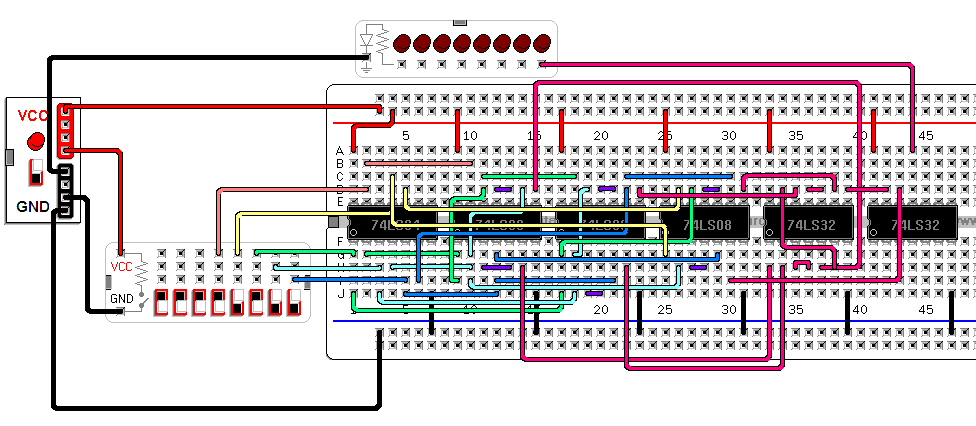
\includegraphics[width=.65\textwidth]{S11}

	\caption{\# 11 Entradas: 0,1,0,1,1 Salida: 0}
\end{figure}

\vspace{.5cm}

\begin{figure}[ht!]
	\centering

	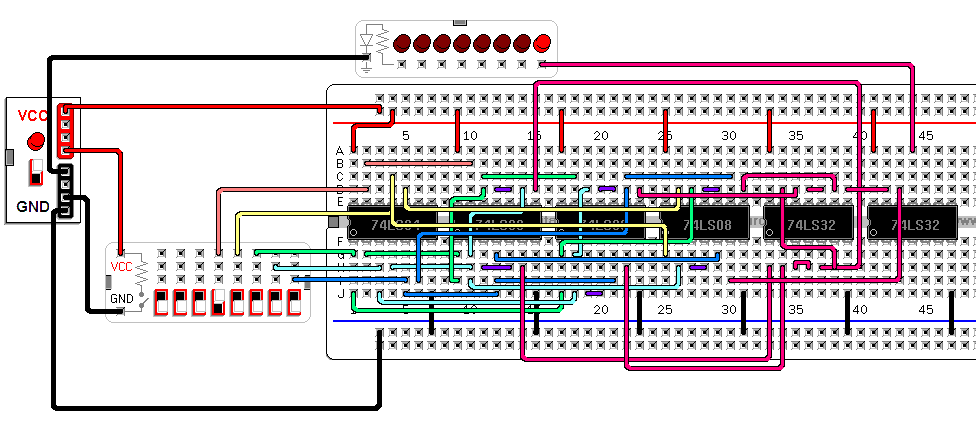
\includegraphics[width=.65\textwidth]{S16}

	\caption{\#16 Entradas: 1,0,0,0,0 Salida: 1}
\end{figure}

\vspace{.5cm}

\begin{figure}[ht!]
	\centering

	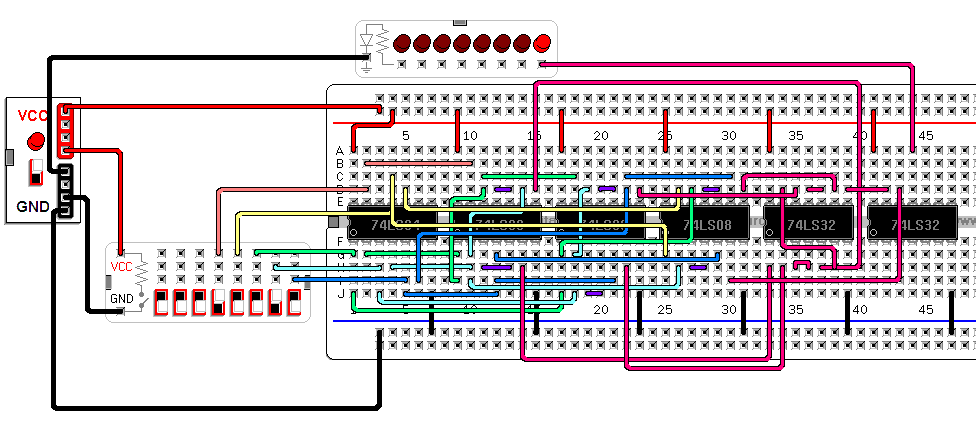
\includegraphics[width=.65\textwidth]{S18}

	\caption{\#18 Entradas: 1,0,0,1,0 Salida: 1}
\end{figure}

\vspace{.5cm}

\begin{figure}[ht!]
	\centering

	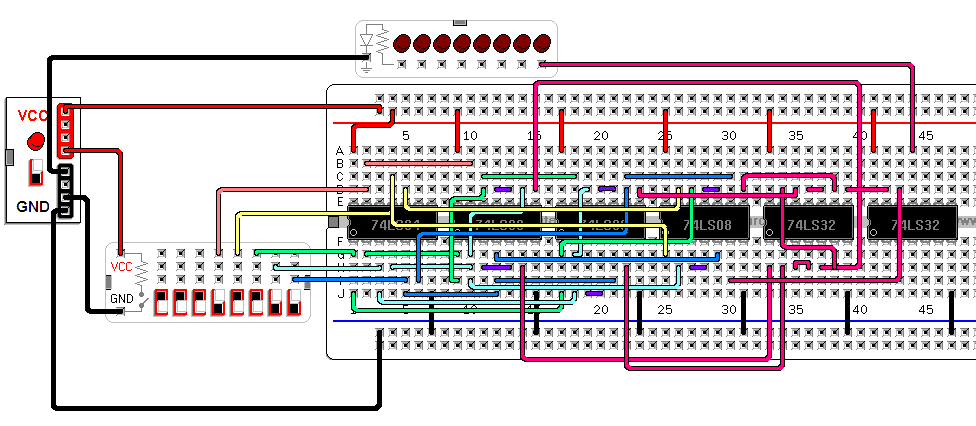
\includegraphics[width=.65\textwidth]{S19}

	\caption{\#19 Entradas: 1,0,0,1,1 Salida: 0}
\end{figure}

\vspace{.5cm}

\begin{figure}[ht!]
	\centering

	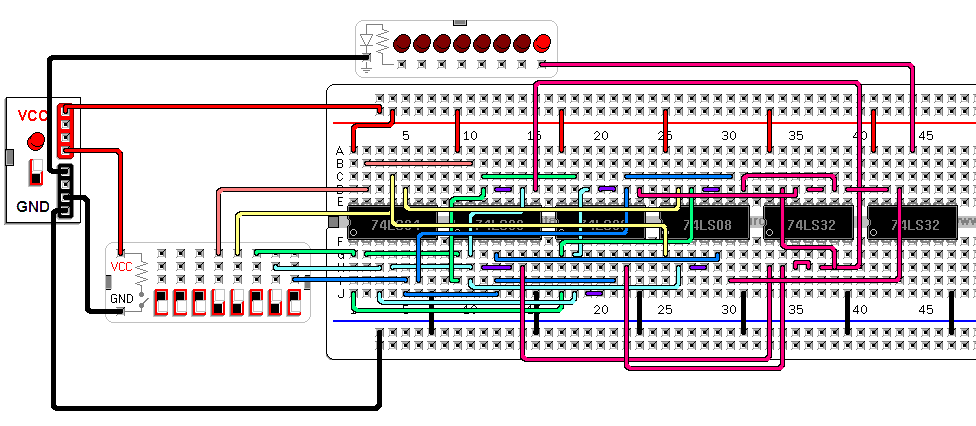
\includegraphics[width=.65\textwidth]{S26}

	\caption{\#26 Entradas: 1,1,0,1,0 Salida: 1}
\end{figure}

\vspace{.5cm}

\begin{figure}[ht!]
	\centering

	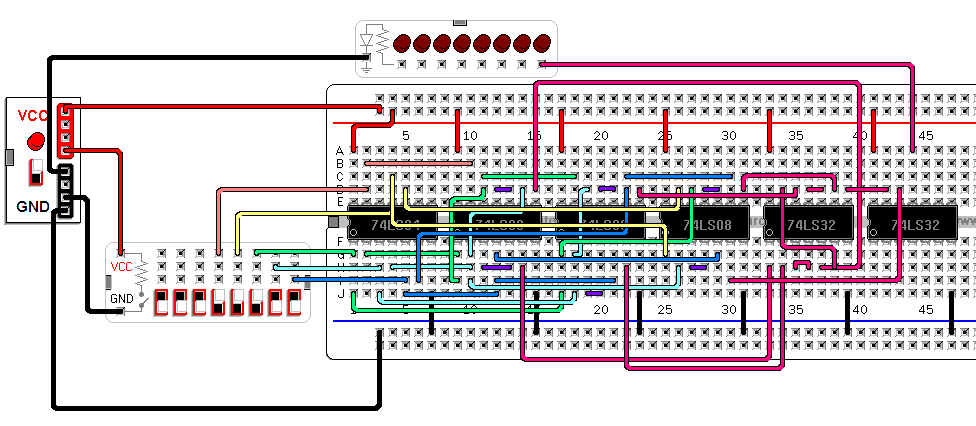
\includegraphics[width=.65\textwidth]{S28}

	\caption{\#28 Entradas: 1,1,1,0,0 Salida: 0}
\end{figure}

\vspace{.5cm}

\begin{figure}[ht!]
	\centering

	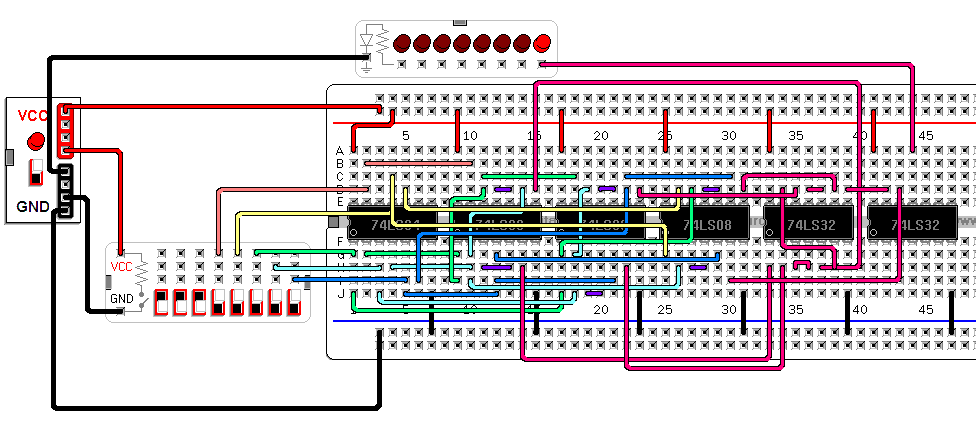
\includegraphics[width=.65\textwidth]{S31}

	\caption{\#31 Entradas: 1,1,1,1,1 Salida: 1}
\end{figure}

\clearpage

%
%
%		CONCLUSIONES
%
%
\newpage
\section{Observaciones y conclusiones}

González Cárdenas Ángel Aquilez

\begin{quotation}
	Al finalizar la practica, se hizo clara la facilidad de utilizar el método del mapa de Karnaugh para simplificar expresiones lógicas. Este método proporciona una forma intuitiva de identificar patrones y agrupar términos para simplificar las funciones booleanas en equivalentes que utilicen menos componentes. \par

	Si bien, es claro que no existe una forma estricta para aplicar el metodo, mientras los resultados en las tablas de verdad sean los mismos o sus equivalentes, también se puede hacer uso de las leyes del algebra booleana para reducir aun mas los componentes a utilizar.

\end{quotation}

\vspace{1cm}

Hernández Reyes Diego Alberto

\begin{quotation}
	En la práctica, se observó la importancia de agrupar los términos \emph{don't care} en el mapa de Karnaugh para lograr una simplificación óptima de la expresión lógica. Al aprovechar los valores \emph{don't care o no importa}, fue posible reducir aún más la complejidad de la función booleana. Esto demostró que, en ciertos casos, el mapa de Karnaugh puede proporcionar simplificaciones más efectivas que las leyes de álgebra booleana y DeMorgan, especialmente cuando se trabajan con circuitos lógicos con multiples entradas o valores de salida inutilizados. Se destacó la importancia de considerar y utilizar cuidadosamente los valores al aplicar el método del mapa de Karnaugh en el diseño de circuitos lógicos ya que los valores a elegir pueden alterar la función original.


	En conclusión, la construcción de circuitos a partir de expresiones simplificadas es esencial para lograr diseños de circuitos eficientes y con el menor número de elementos necesarios.\par
\end{quotation}


\end{document}